% !TEX TS-program = pdflatex
% !TEX encoding = UTF-8 Unicode

% This is a simple template for a LaTeX document using the "article" class.
% See "book", "report", "letter" for other types of document.

\documentclass[11pt]{article} % use larger type; default would be 10pt

\usepackage[utf8]{inputenc} % set input encoding (not needed with XeLaTeX)

%%% Examples of Article customizations
% These packages are optional, depending whether you want the features they provide.
% See the LaTeX Companion or other references for full information.

%%% PAGE DIMENSIONS
\usepackage{geometry} % to change the page dimensions
\geometry{a4paper} % or letterpaper (US) or a5paper or....
% \geometry{margin=2in} % for example, change the margins to 2 inches all round
% \geometry{landscape} % set up the page for landscape
%   read geometry.pdf for detailed page layout information

\usepackage{graphicx} % support the \includegraphics command and options

% \usepackage[parfill]{parskip} % Activate to begin paragraphs with an empty line rather than an indent

%%% PACKAGES
\usepackage{booktabs} % for much better looking tables
\usepackage{array} % for better arrays (eg matrices) in maths
\usepackage{paralist} % very flexible & customisable lists (eg. enumerate/itemize, etc.)
\usepackage{verbatim} % adds environment for commenting out blocks of text & for better verbatim
\usepackage{subfig} % make it possible to include more than one captioned figure/table in a single float
% These packages are all incorporated in the memoir class to one degree or another...

%%% HEADERS & FOOTERS
\usepackage{fancyhdr} % This should be set AFTER setting up the page geometry
\pagestyle{fancy} % options: empty , plain , fancy
\renewcommand{\headrulewidth}{0pt} % customise the layout...
\lhead{}\chead{}\rhead{}
\lfoot{}\cfoot{\thepage}\rfoot{}

%%% SECTION TITLE APPEARANCE
\usepackage{sectsty}
\allsectionsfont{\sffamily\mdseries\upshape} % (See the fntguide.pdf for font help)
% (This matches ConTeXt defaults)

%%% ToC (table of contents) APPEARANCE
\usepackage[nottoc,notlof,notlot]{tocbibind} % Put the bibliography in the ToC
\usepackage[titles,subfigure]{tocloft} % Alter the style of the Table of Contents
\renewcommand{\cftsecfont}{\rmfamily\mdseries\upshape}
\renewcommand{\cftsecpagefont}{\rmfamily\mdseries\upshape} % No bold!

\usepackage{hyperref}
\usepackage{mathtools}
\usepackage[usenames,x11names,table]{xcolor}
\usepackage{minted}
\usepackage{tikz}
\usepackage{draftwatermark}
\SetWatermarkScale{5}
%%% END Article customizations

%%% The "real" document content comes below...

\title{Solve Weighing Pool Ball Puzzle}
\author{Szabolcs Seláf \\ \texttt{selu@selu.org}}
%\date{} % Activate to display a given date or no date (if empty),
         % otherwise the current date is printed 

\begin{document}
\maketitle

\section{Weighing Pool Ball Puzzle}

The problem is described at \url{https://www.mathsisfun.com/pool_balls.html} with a solution. But the given solution is undetermined. Subsequent measures are depends on the result of the previous one. Ferenc Rákóczi mentioned, he already had a determined solution for this problem, but he forgot it.

\subsection{The problem}

You have 12 balls identical in size and appearance but 1 is an odd weight (could be either light or heavy).

You have a set of balance scales which will give 3 possible readings:

\begin{itemize}
\item Left $=$ Right
\item Left $>$ Right
\item Left $<$ Right (ie Left and Right have equal weight, Left is Heavier, or Left is Lighter).
\end{itemize}

You have \emph{only 3 chances} to weigh the balls in any combination using the scales.
Find which ball is the odd one and if it's heavier or lighter than the rest.

\section{Find one solution}

\subsection{Generate possible measures}
At first I calculated the number of possible measures. We should put equal number of balls onto both arms to get a valid result, so pick even number of balls for measure, then pick half of the balls for Left arm and put remaining balls into Right arm. We can halve the numbers, because putting same set of balls to Right arm is same as to Left arm:

\[ \sum_{i=1}^{6} \frac{\binom{12}{2i} \binom{2i}{i}}{2} = 36829 \]

All three measures can be one of the 36829 possible ones, so the number of all possible solutions could be:

\[ 36829^3 = 49953943750789 \]

Using information above we can generate possible measures one-by-one:

\begin{minted}{ruby}
ids = (1..12).to_a                          # array [1, 2, .., 12] for balls
(1..6).each do |level|                      # how much balls to put on an arm
  ids.combination(level*2).each do |subset| # pick a combination for both arms
    reverse = []
    subset.combination(level).each do |left| # pick half of them for left arm
      next if reverse.include?(left)         # go to next if reversed already
      right = subset - left                  # checked
      reverse << right
\end{minted}

\subsection{Backtracking}

At start any of the 12 balls can be heavier or lighter than others, which means we have 24 possible results. Each measure has 3 possible outcomes, 3 measures could solve $3^3 = 27$ different cases. After the first measure the remaining two could solve only $3^2 = 9$ cases and of course, the last one could solve maximum 3 cases.

The program uses this knowledge to give up, once there is a possible outcome of a measure with more different cases, than that can be eliminated by the remaining steps.

\begin{minted}{ruby}
if state_set.map(&:case_number).max > (Scale.number_of_outcomes ** max_measures)
  return
end
\end{minted}

\subsection{Result}

However this algorithm is almost a brute force, found the first solution within some seconds.

\begin{table}[ht]
\begin{center}
\begin{tabular}{|c|cccc|cccc|}
  \hline
  Number & \multicolumn{4}{c|}{Left arm} & \multicolumn{4}{c|}{Right arm} \\
  \hline
       1 & 1 & 2 & 3 & 4 & 5 & 6 & 7 & 8 \\
       2 & 1 & 2 & 3 & 5 & 4 & 9 & 10 & 11 \\
       3 & 1 & 4 & 6 & 9 & 2 & 7 & 10 & 12 \\
  \hline
\end{tabular}
\end{center}
\caption{Measures}
\end{table}

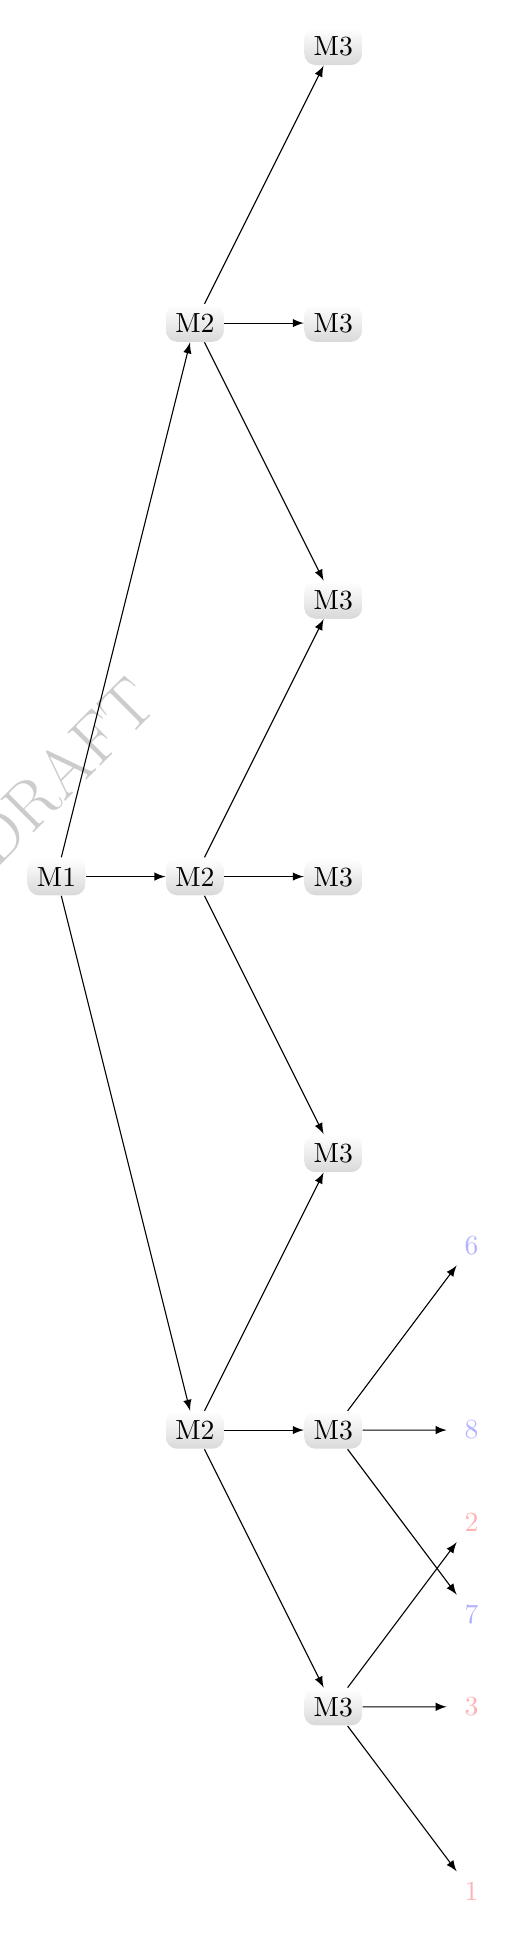
\begin{tikzpicture}
[
  choose/.style     = {shape=rectangle, rounded corners,
                       bottom color=gray!30, top color=white},
  heavy/.style      = {shape=circle, color=red!30},
  light/.style      = {shape=circle, color=blue!30},
  edge from parent/.style = {draw, -latex},
  grow = right,
  level/.style =    { level distance=5em, sibling distance=20em/#1 }
]
\node [choose] {M1}
  child { node [choose] {M2}
    child { node [choose] {M3}
      child { node [heavy] {1} }
      child { node [heavy] {3} }
      child { node [heavy] {2} }
    }
    child { node [choose] {M3} 
      child { node [light] {7} }
      child { node [light] {8} }
      child { node [light] {6} }
    }
    child { node [choose] {M3} 
    }
  }
  child { node [choose] {M2}
    child { node [choose] {M3} }
    child { node [choose] {M3} }
    child { node [choose] {M3} }
  }
  child { node [choose] {M2}
    child { node [choose] {M3} }
    child { node [choose] {M3} }
    child { node [choose] {M3} }
  }
  ;
\end{tikzpicture}

\end{document}
